% !TEX root = ./main.tex
\section{Experimental results}
\label{sec:experiments-cs}
Our experiments focus on the following questions:
\begin{enumerate}
\item \textbf{Finding critical clusters.} Can we find highly critical regions with our proposed methods? How do they compare to standard baselines used in public health? (Section \ref{sec:opt-power})
\item \textbf{Characteristics of critical clusters.} What are the demographic properties of critical clusters? Where are they located? (Section \ref{sec:demographics})
%\item \textbf{\maxcrit{} vs.\ \avgcrit{}.} What are the differences and similarities of the clusters discovered under the two proposed problems? (Section \ref{sec:compare-formulations})
\end{enumerate}

\subsection{Experimental Setup}
\subsubsection{Dataset and disease model.}
\label{sec:data}
A study of epidemics that spread through physical proximity requires social contact networks in which an edge represents physical contact
between two people at some location during the day. Such networks cannot be constructed easily because of the difficulty in tracking contacts for a large set of people.
This has been recognized as a significant challenge in the public health community,
and multiple methods have been developed to construct realistic contact
network models by integrating diverse public datasets
(e.g., US Census, land use, and activity surveys) and
commercial data (e.g., from Dunn \& BradStreet on location profiles).
We use models developed by the approach of 
\cite{eubank:nature04}; %\footnote{See \url{ndssl.vbi.vt.edu/synthetic-data/download}
%for networks available for download.}
see also \cite{longini05:science,fc+06} for network
models developed by other public health groups. %\footnote{Models are available at
%\url{http://www.epimodels.org/drupal/?q=node/70} and
%\url{https://www.rti.org/impact/synthpop}}
Multiple such network models were evaluated in a study by the Institute of Medicine
\cite{halloran:pnas08}.

Here, we focus on a population for Minnesota with $5,048,920$ individuals in total, aggregated into 4,082 census block groups from the 2010 U.S. census. 
We consider an SEIR  stochastic model for measles, as described in
Section \ref{sec:background}.
The criticality of a region $R$ of block groups is assessed by leaving 
every individual inside $R$ unvaccinated; everybody else in the population 
is vaccinated with probability 0.97, which is the statewide vaccination rate. %The
%source $\src$ is as a set of three nodes in $\mathcal{C}$ selected uniformly at random.
%For the \avgcrit{} formulation, we focus on the Minneapolis metropolitan area and
%pick $\src$ to be a set of 100 children selected uniformly at random.
%As before, we assess the criticality of a cluster by leaving its inhabitants unvaccinated, with a %0.97 vaccination rate elsewhere. 
%%The difference between \avgcrit{} and \maxcrit{} is that the seeds are pre-selected and unchanged in the former, but they are selected from the cluster under evaluation in the latter. We assume vaccinations with high efficacy, which is the case for MMR, the measles vaccine.

%%%%%For the \maxcrit{} formulation, the criticality of a cluster of block groups is assessed by leaving every individual inside the cluster unvaccinated; everybody else in the population is vaccinated with probability 0.97, which is the statewide vaccination rate. Then, we select 3 random individuals as ``seeds'' of the infection and simulate 400 days of disease spread. For the \avgcrit{} formulation, we focus on the Minneapolis metropolitan area. First, we randomly select 100 individuals as seeds of the infection; these stay fixed throughout different runs of the simulation. As before, we assess the criticality of a cluster by leaving its inhabitants unvaccinated, with a 0.97 vaccination rate elsewhere. The difference between \avgcrit{} and \maxcrit{} is that the seeds are pre-selected and unchanged in the former, but they are selected from the cluster under evaluation in the latter. We assume vaccinations with high efficacy, which is the case for MMR, the measles vaccine.

%
%\subsubsection{Dataset and Simulation Engine}
%\label{sec:data}
%A study of epidemics that spread through physical proximity
%requires social contact networks in which an edge represents an actual physical contact
%between two people at some location during the day. Such networks are
%not readily available and cannot be constructed easily
%because of the difficulty in tracking individuals' contacts over a day on a reasonable scale.
%We study a specific class of realistic population and social contact graphs
%developed using first principles based methods \cite{barrett:wsc09,eubank:nature04}.
%We briefly summarize how these networks are constructed, and refer to
%\cite{barrett:wsc09,eubank:nature04} for the details.
%(i) A synthetic urban population model is constructed by integrating over a dozen
%public data (e.g., US Census, land use and activity surveys) and
%commercial data (e.g., from Dunn \& BradStreet on location profiles). The resulting
%population is statistically equivalent to the census;
%(ii) A sequence of activities is constructed for each household and each person---this
%models the type of activity performed by each person, along with other attributes,
%such as duration. The activities of different members of the same household are correlated;
%(iii) Activity locations are assigned for each person, using land use data and
%activity choice models; and
%(iv) Individuals are routed through the road network, which in turn gives a
%social contact network based on co-location. These network models have been used
%in a number of studies on epidemic spread and public health policy planning---see, e.g.,
%\cite{eubank:nature04, saha:sdm15, barrett:wsc09, bisset09epifast, dblp:conf/sbp/chenmm10}.
%
%In particular, we focus on a synthetic population of Minnesota, which has $5,048,920$ agents in total.
%These agents are aggregated into 4,082 census block groups from the 2010 U.S. census.
%Using the EpiFast simulation engine \cite{bisset09epifast}, we simulate 400 days of the spread of a
%disease with an attack rate of $45\%$, following the SIR model. In order to estimate the criticality of
%a subgraph, we run the simulation 100 times.
%%We experiment with different vaccination interventions in the population. In the experiments
%%below, an $x\%$ vaccination compliance means that every person in the population is vaccinated with
%%probability $x / 100$.

\subsubsection{Baseline Methods}
We compare our algorithms with two heuristics used in public health and a naive random baseline.
\begin{enumerate}
\item \textsc{Population.} Find a cluster of size $k$ with the largest total population.
The motivation behind this heuristic is leaving as many people as possible unvaccinated.

\item \textsc{Vulnerability.} The vulnerability of an individual is the probability that this person will get infected when the disease is left to propagate with no intervention---i.e., $x_v = 0$ for all nodes. This baseline finds a cluster of size $k$ with as large total vulnerability as possible, thus prioritizing individuals who are most likely to get infected. 
\item \textsc{Random.} Find a connected cluster of size $k$ by doing a random walk on the auxiliary graph $\HR$.
\end{enumerate}

\subsection{Optimization power}
\label{sec:opt-power}
In Figure \ref{fig:cri-baseline-compare}, we show the criticality obtained by \algomaxcrit{} compared to the three baseline methods as a function of $k$. As expected, selecting subgraphs at random performs poorly and results in almost no additional infections compared to the initial disease conditions. Surprisingly, \textsc{Vulnerability} does not perform much better than \textsc{Random}. It is also interesting that the population-based heuristic does not have monotonic improvement with $k$. Even though the subgraph of size 9 has 55,800 inhabitants, the smaller subgraph of size 5 with a population of 34,000 leads to a much larger outbreak. 
Overall, the \textsc{Population} heuristic has better performance among the baselines, and it even surpasses our algorithm for $k=5$. However, \algomaxcrit{} exhibits notably better performance in general. The maximum improvement on criticality occurs on the 9-node cluster, where our method finds a cluster that leads to 4 times more infections than the \textsc{Population} baseline.

\begin{figure}
\centering
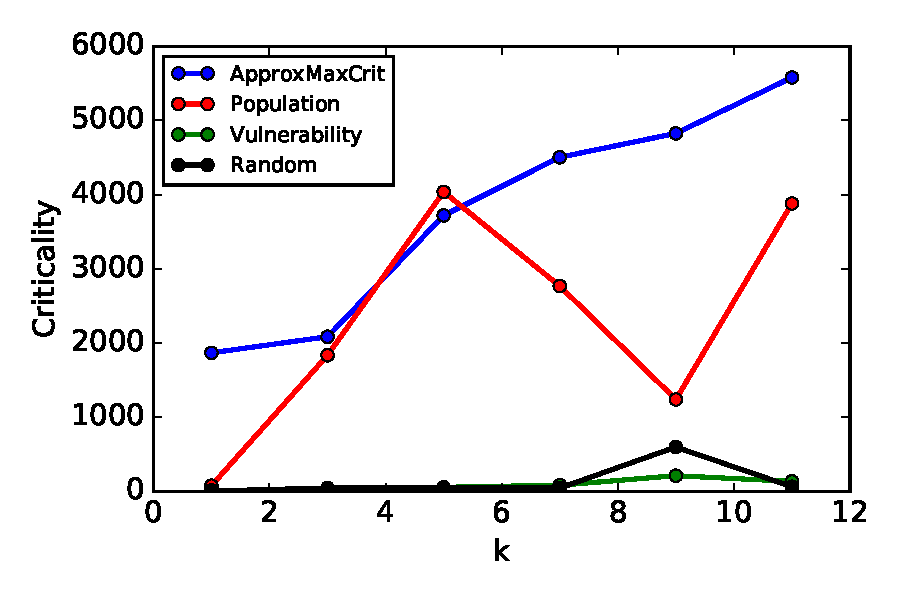
\includegraphics[width=.35\textwidth]{img/criticality-baseline-comparison.pdf}
\vspace{-.2in}
\caption{Comparison of algorithms for the \maxcrit{} problem as a function of the solution size $k$}
\label{fig:cri-baseline-compare}
\end{figure}

Another important quantity is the probability of having a large outbreak.
In Figure \ref{fig:crit-boxplots}, we show the distribution of criticality values 
for each method over 100 simulations of the disease model.
We observe that even the largest outbreaks caused by \textsc{Vulnerability} and \textsc{Random} are much smaller than those of \algomaxcrit{} and the \textsc{Population} baseline. We also note that the population-based clusters have larger variance in criticality and can result in larger outbreaks than those from our algorithm. This suggests that if the goal for a public health department is to prevent the worst-case scenario, then intervening the most-populated areas is a good heuristic. However, in doing so, one could miss smaller regions that, on average, are likely to infect more people.
%We report similar results on optimization power for \algoavgcrit{} in the Supplementary Material.

\begin{figure*}
\centering
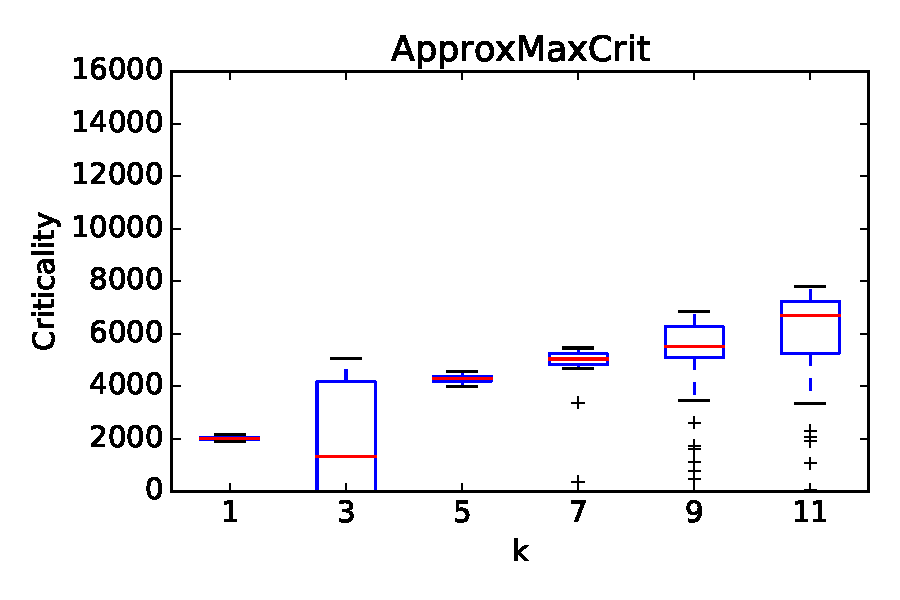
\includegraphics[width=0.24\textwidth]{img/mn_criticality_cluster_boxplot.pdf}
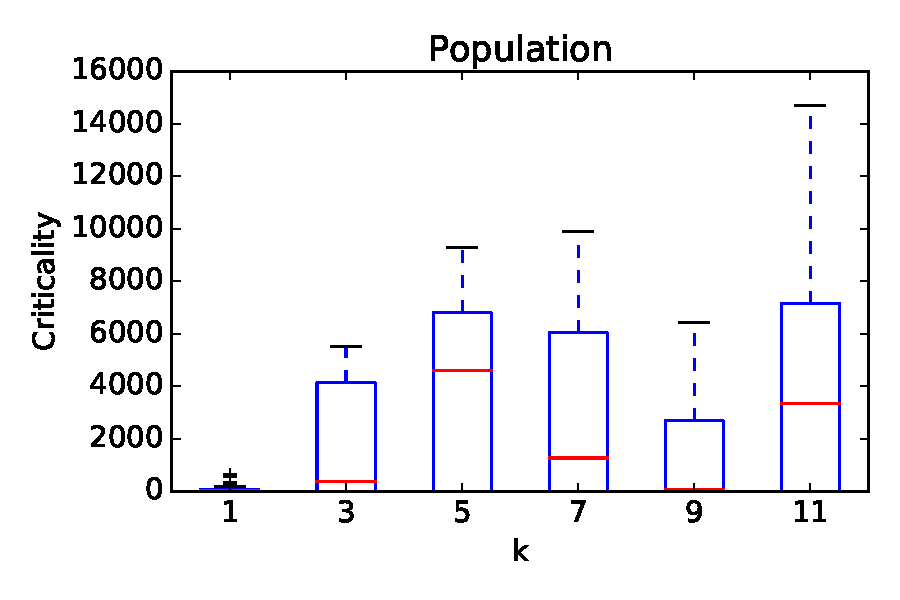
\includegraphics[width=0.24\textwidth]{img/mn_popsize_cluster_boxplot.pdf}
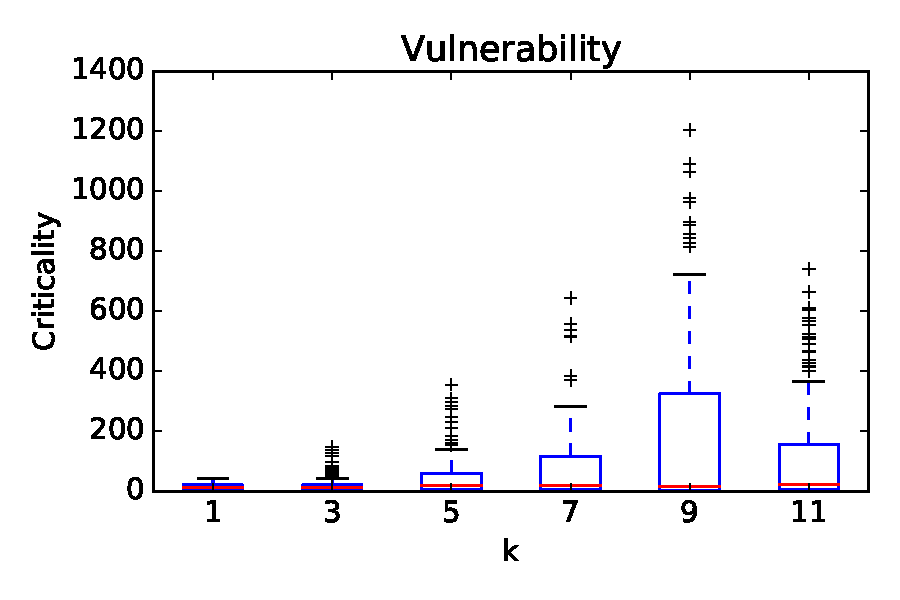
\includegraphics[width=0.24\textwidth]{img/mn_avg_blkgrp_cluster_boxplot.pdf}
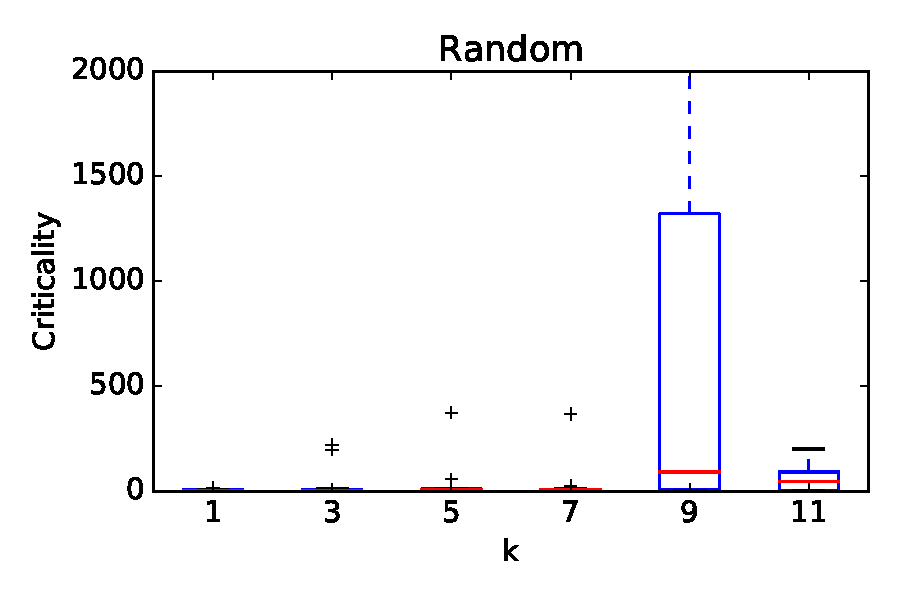
\includegraphics[width=0.24\textwidth]{img/mn_random_blkgrp_cluster_boxplot.pdf}\\
\caption{Criticality scores over 100 runs of the disease model for each method evaluated}
\label{fig:crit-boxplots}
\end{figure*}

\subsection{Critical clusters and demographics}
\label{sec:demographics}
We compare the distribution of age and income in the cluster discovered by \algomaxcrit{} ($k=11$) to that of the entire state. We aggregate household income into ``Low'' (below \$25,000), ``Medium'' (between \$25,000 and \$75,000), and ``High'' (above \$75,000). Ages are binned into ``Pre-school'' (below 5 years old), ``School'' (between 5 and 18 years old), ``Adult'' (between 18 and 70 years old), and ``Senior'' (above 70 years old). In Figure \ref{fig:cluster-demographics}, we see the critical cluster has significantly more households of low income compared to the entire state---19.6\% to 34.9\%. Similarly, children are over-represented. 26.6\% of the population are children in ``School'' age compared to the average of 18.7\%.

\begin{figure}
\centering
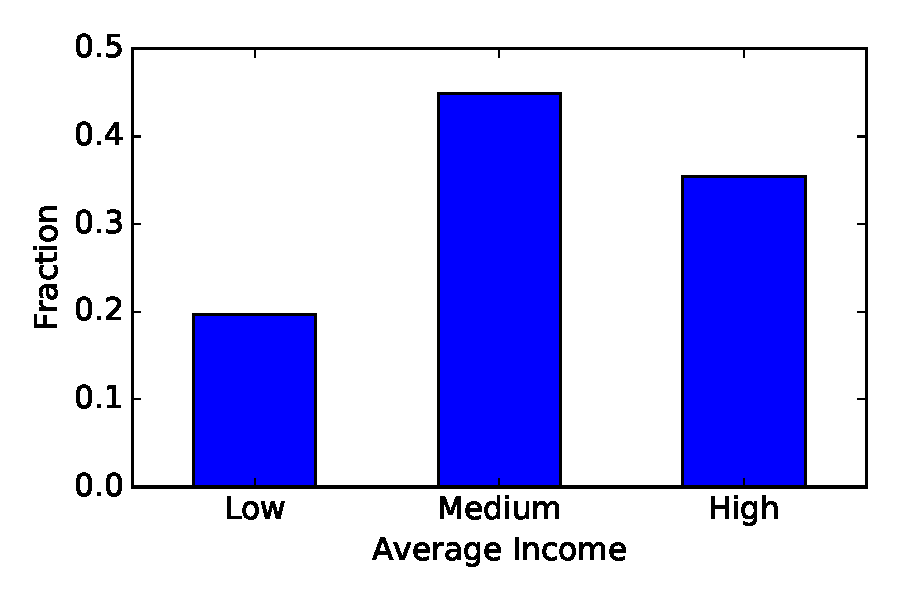
\includegraphics[width=0.23\textwidth]{img/mn-income.pdf}
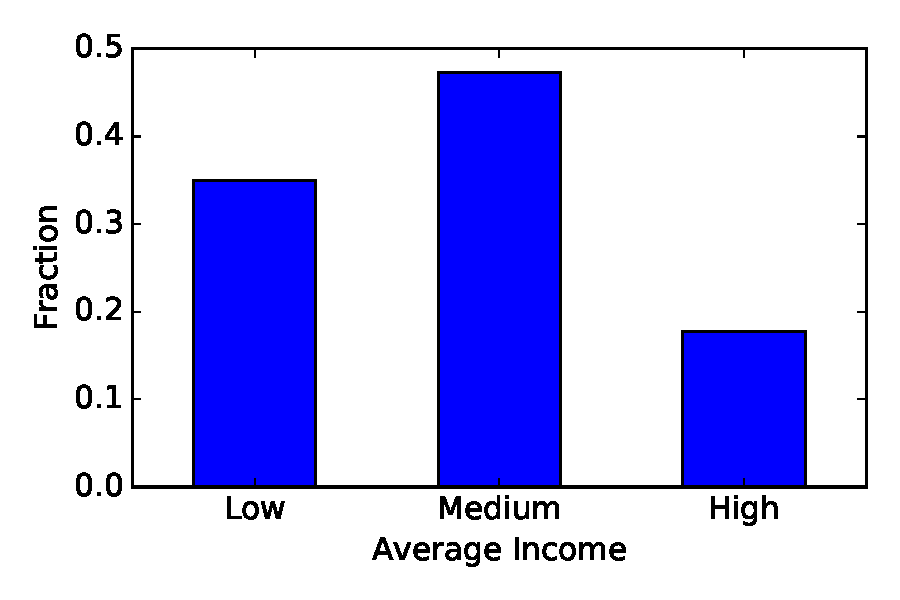
\includegraphics[width=0.23\textwidth]{img/kmaxst-11-income.pdf}
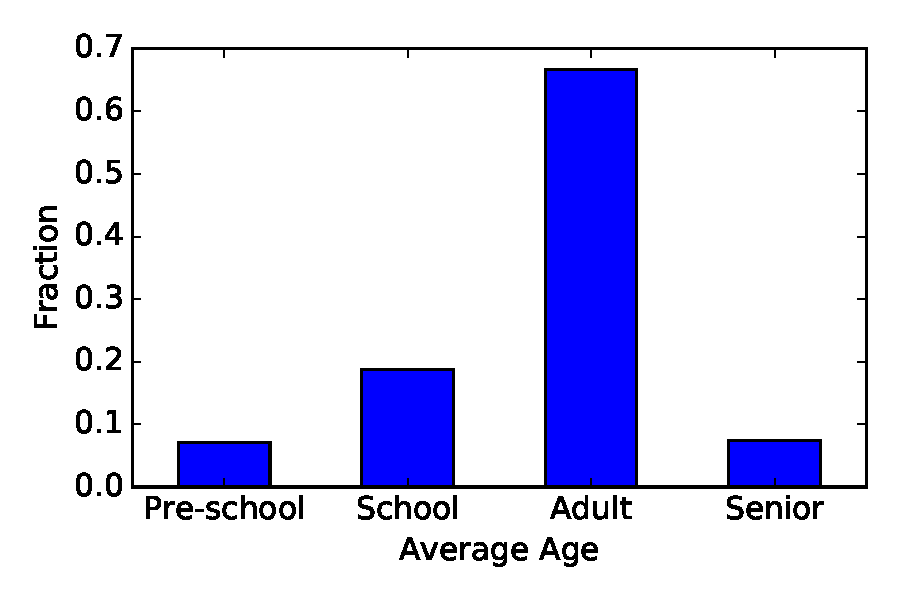
\includegraphics[width=0.23\textwidth]{img/mn-age.pdf}
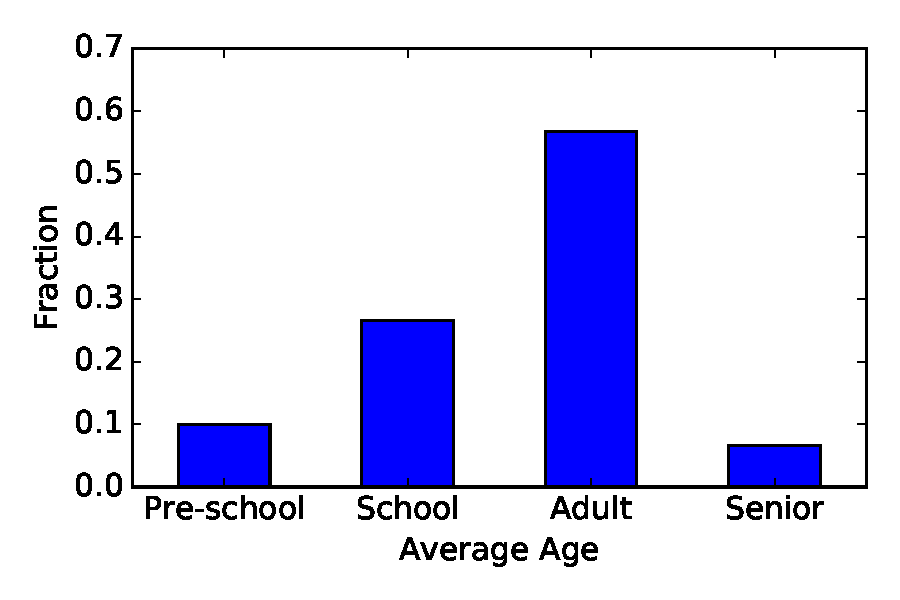
\includegraphics[width=0.23\textwidth]{img/kmaxst-11-age.pdf}
\caption{Average income (top) and age (bottom) in the entire state (left) and in the cluster discovered by \algomaxcrit{} (right). There are more children in school age and lower income households in the discovered critical cluster.}
\label{fig:cluster-demographics}
\end{figure}

We find critical clusters in different regions over Minnesota. Figure \ref{fig:mn-criticalsets} shows the top 10 non-overlapping clusters discovered using \algomaxcrit{}. The most critical cluster---with over 5,000 infections---is located on the rural northern part of the state, spanning the Leech Lake and Red Lake reservations. We note that this cluster results in the largest spread despite having a relatively small population of 14,910 people compared to clusters in urban regions. For example, the second most critical cluster---north of Minneapolis---has 48,889 inhabitants. %One possible explanation is that the largest cluster spans a larger geographical area, which could make the criticality function in that region closer to being modular than submodular. 

In addition to analyzing the most critical cluster, we look at the top-5 non-overlapping clusters discovered by \algomaxcrit{}. These correspond to different choices of root on the k-\textsc{MaxST} algorithm. In Table \ref{tab:top5-scores}, we report the total population size, criticality, and percentage of infections to the total population of the cluster---i.e., criticality / population. Note that this latter number could be larger than 1, since there are infections outside the cluster. As we discussed before, the top region leads to a large spread (41\% of its population size) despite having less inhabitants than the successive clusters. The second cluster has very similar criticality score, but in a more urban region.

\begin{table}
\centering
\caption{Total population and criticality in the top 5 clusters discovered by \algomaxcrit{}
%\vspace*{-.15in}
}
\label{tab:top5-scores}
\begin{tabular}{|c|r|r|r|}
\hline
\textbf{Rank} & \textbf{Population} & \textbf{Criticality} & \textbf{\% population}\\
\hline
1 & 14,910 & 6,138 & 41.2\%\\
2 & 48,889 & 6,093 & 12.5\%\\
3 & 23,391 & 1,388 & 5.9\%\\
4 & 15,731 &   647 & 4.1\%\\
5 &  9,936 &   372 & 4.7\%\\
\hline
\end{tabular}
\end{table}

Finally, we repeat our experiments for \maxcrit{} on the Minneapolis area instead of the entire state. The most critical cluster covers Brooklyn Park, where measles outbreaks occurred in 2017 and 2019\footnote{\url{https://tinyurl.com/y359zapv}}. However, we emphasize the need for domain-expert analysis to better interpret and make use of these results.
%, highlighted in red in Figure \ref{fig:brooklyn-park}, covers Brooklyn Park, where measles outbreaks occurred in 2017 and 2019\footnote{\url{https://tinyurl.com/y359zapv}}. However, we emphasize the need for domain-expert analysis to better interpret and make use of these results.

%\begin{figure}
%\centering
%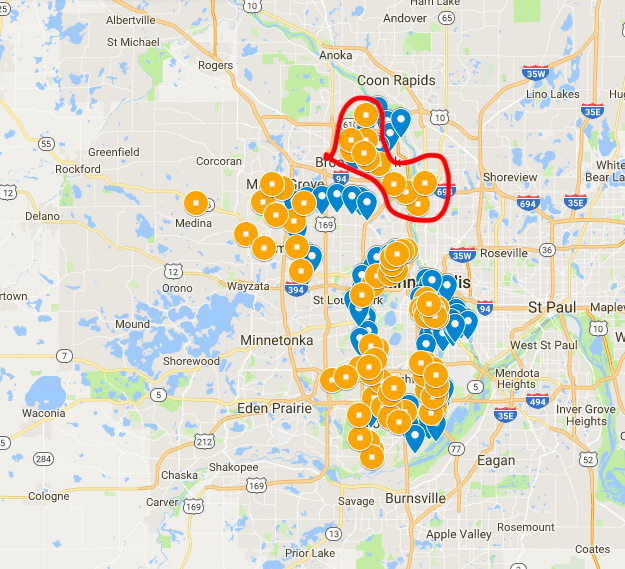
\includegraphics[width=0.4\textwidth]{img/maxcrit_minneapolis_clusters_higlighted.png}
%\caption{\maxcrit{} clusters in Minneapolis. Most critical cluster (highlighted in red) covers Brooklyn Park.}
%\label{fig:brooklyn-park}
%\end{figure}

%\begin{figure}
%\centering
%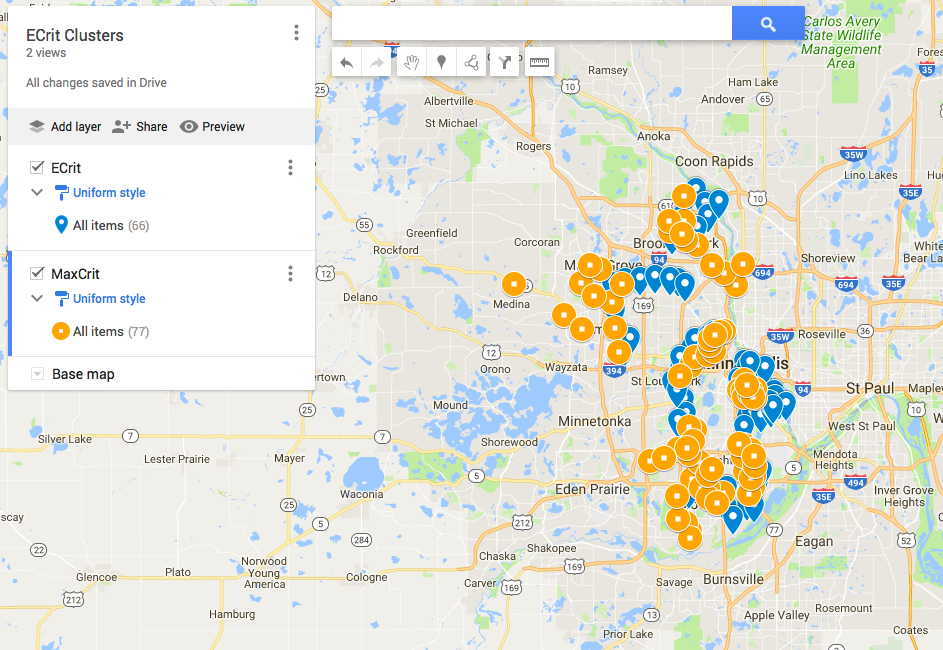
\includegraphics[width=0.4\textwidth]{img/maxcrit_minneapolis_clusters.png}
%\caption{\maxcrit{} and \avgcrit{} clusters in Minneapolis. Both solutions find similar critical clusters.}
%\label{fig:both-clusters}
%\end{figure}

%\subsection{\avgcrit}
%\begin{figure}
%\centering
%\includegraphics[width=.45\textwidth]{img/ecrit-baseline-comparison.pdf}
%\vspace{-.2in}
%\caption{Comparison of algorithms for \avgcrit{} as a function of the solution size $k$}
%\label{fig:ecrit-baseline-compare}
%\end{figure}


%\subsection{Criticality Based on Vulnerability}
%First, we study the criticality of the critical regions discovered by maximizing vulnerability. In Figure \ref{fig:cri-set-k12}, we observe the effect of leaving the most vulnerable region unvaccinated as a function of compliance in that region, for a region size of $k=12$. If the region is left unvaccinated, we observe a substantial outbreak. Even if the rest of the population is well-vaccinated (i.e., rates of 80\%, 90\%, and 95\%), the disease still affects tens of thousands of people, corresponding to at least 1\% of the population. In fact, we need at least 50\% compliance on the critical region to stop the disease from taking off.

%\begin{figure}
%\includegraphics[scale=.5]{img/vulnerable-ct-compliance-k12-rate.pdf}
%\includegraphics[scale=.5]{img/vulnerable-ct-compliance-k12-counts.pdf}
%\caption{If a subgraph with high vulnerability has low vaccination compliance (less than 50\%), we observe a substantial outbreak even if the rest of the population has high compliance (80\%, 90\%, and 95\%).}
%\label{fig:cri-set-k12}
%\end{figure}
%
%In Figure \ref{fig:cri-set-k3}, we observe a similar effect even for a critical set of only 3 census tracts ($k=3$).
%
%\begin{figure}
%\includegraphics[scale=.5]{img/vulnerable-ct-compliance-k3-rate.pdf}
%\includegraphics[scale=.5]{img/vulnerable-ct-compliance-k3-counts.pdf}
%\caption{Same as Figure \ref{fig:cri-set-k12} but for $k=3$. Even for a set of only 3 census tracts, we observe an outbreak on the order of $10^5$ infections when the critical set has low compliance.}
%\label{fig:cri-set-k3}
%\end{figure}

%\begin{figure}
%\centering
%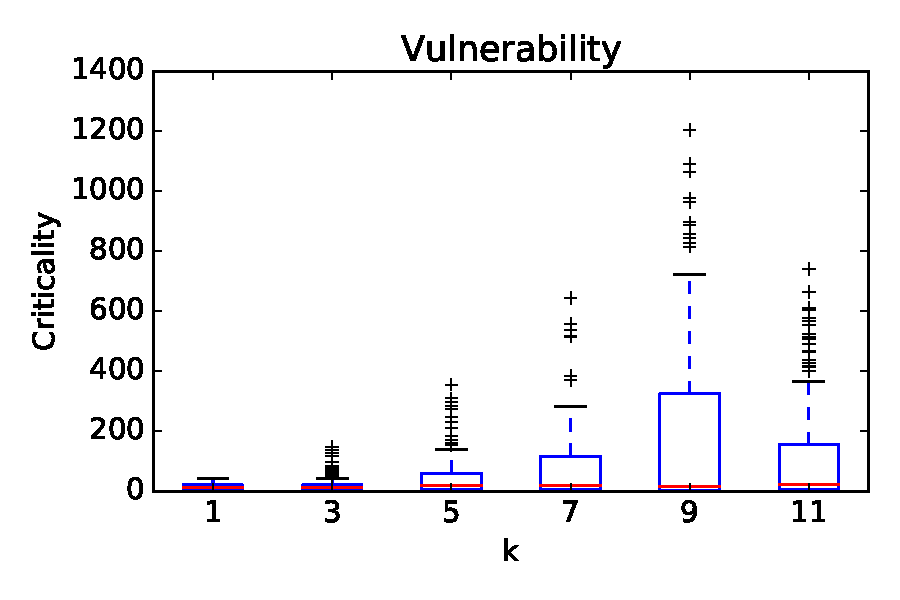
\includegraphics[scale=.5]{img/mn_avg_blkgrp_cluster_boxplot.pdf}	
%\includegraphics[scale=.5]{img/random-clusters-mn-blkgrp-boxplot.pdf}
%\caption{Distribution of criticality over multiple simulations.}
%\label{fig:cri-boxplots}
%\end{figure}
%
%
%\subsection{Comparison to random subgraphs.} In order to compare our algorithm based on maximizing vulnerability, we compare the graph that we found with 100 randomly sampled connected subgraphs. In Figure \ref{fig:cri-random}, we show the distribution of number of infections of this random subgraphs for a compliance rate of 95\% in the population outside the subgraph---left is for $k=12$ and right is for $k=3$. We find that our algorithm discovers a subgraph that is in the 99th percentile of this distribution; further, the subgraph that scores higher than our method has high overlap with the subgraph we discover. Thus, maximizing vulnerability is a strong heuristic for criticality.

%\begin{figure}
%\centering
%\includegraphics[scale=.5]{img/random-ct-compliance95-k12-counts.pdf}
%\includegraphics[scale=.5]{img/random-ct-compliance95-k3-counts.pdf}
%\caption{Distribution of attack rates in 100 random subgraphs of 12 (left) and 3 (right) random connected subgraphs. 99\% of the time maximizing modularity performs better.}
%\label{fig:cri-random}
%\end{figure}

%\subsection{Locations of Critical Regions}
%In Figure \ref{fig:critical-seattle}, we show the locations of the 10 regions with highest vulnerability in the Seattle dataset. Critical regions correspond to eithe 1) highly populated places, and 2) places with many children.
%
%\begin{figure}
%\centering
%\includegraphics[scale=.35]{img/critical-sets-k3-markers.png}
%\caption{Locations of the 10 subsets of size 3 with highest vulnerability. The stars mark the subset with highest vulnerability.}
%\label{fig:critical-seattle}
%\end{figure}
